\section{Optimization Techniques}
In this section, we briefly analyze some possible improvements to the CPU emulation of the emulator, then we will show which of the optimizations we made and optimizations that we tried to implement but didn't work.

\subsection{Pre-decoding}
Every time the emulator prepares to execute the next instruction, it needs to perform multiple accesses to the memory in order to get all the necessary values to execution of the instruction. For instance, when trying to load a value to a register, the emulator needs to get the opcode of the instruction pointed by the program counter, then read the value of the register and last, read the value. This could be avoided if every time the emulator is reading from a new memory position that was never executed before, it saved the unchanged values, like the opcode and the register number into a cache. The next time this instruction would be performed, less memory accesses would be needed, improving the emulator's performance.\\
\indent We tried this approach, but due to the paging mechanism of the emulator, the cache needed to be cleaned every time a page changed occurred.

\subsection{Indirect Threading}
For each execution of the decode loop, the emulator uses an enormous switch/case statement to match and execute and instruction. this bad in terms of code location because we are constantly jumping between distinct code zones. It could be avoided if in the end of each instruction, the emulator seek on a table which would be the next instruction to be executed, jump to it and execute it.

\subsection{Switch/case removal}
As we said, each time an instruction is to be decoded the emulator performs a comparison of the instruction opcode with all the possible opcodes until it finds a match. We can remove this overhead by having a table of instructions ordered by the opcode. Each time the emulator needs to discover which operation to execute it only needs to access one position of the table and execute the instruction.

\subsection{Lazy flags}
Each time an instruction is executed it updates the values of the affected flags. The work of updating the flags is sometimes bigger than executing the instruction itself and most of the times the flags values are not used. We can remove this source of overhead by calculating the flags in a lazy way. That is, none of the instructions updates the flags and when an instruction need to use a flag value, it calculates the value for that flag.

\subsection{Parallel update and emulate}
In the decode and dispatch loop each time an instruction is executed the emulator updates the screen and makes a sleep to maintain compatibility with the original processor but when it returns from the sleep it need to wait for the instruction to be executed. This work could be made in parallel, that is, we could execute the instruction at the same time we are waiting for the next screen update and with this, when the sleep ends we already have the next instruction executed and we could update and sleep again. With this approach we would have zero time for executing the instructions because that time would be overlapped by the time of sleep and updates.

\subsection{CPU Emulation}
Here, we present all the improvements performed to the emulator. All but one, the last, were implemented successfully, the reasons for that will be addressed later.

\subsubsection{Instructions array}
In the original implementation, each time an instruction is to be decoded it compares the opcode of that instruction with all the possible opcodes. This was done in an enormous switch case that was not even sorted by the most used instructions and so in the worst case the emulator needed to do N comparisons for each original instruction (being N the total number of instructions of the Z80). All the code that implements an instruction was on the respective case statement. This could be good because it has no indirection level for the execution of the instruction code but the number of comparisons and branches that needs to be performed in the switch statement totally overlaps this.\\
\indent As you can intuitively say, this was a major source of inefficiency and so we needed to change the way of decoding an instruction.
We choose to have an array of instructions in witch the position of a given instruction is the same as the opcode for that instruction. this is possible because we only have 255 main instructions. There are some instructions like the EDh FDh and DDh that use a bigger opcode and so we use an extra level of indirection maintaining the switch statement for this kind of instructions. This is not problematic because this instructions are originally the less used.
For each of the main instructions we created a new instruction class with the original code that was on the switch statement and so the behavior was not affected. Each of the positions of the instructions array is an instruction instance that knows how to emulate the original instruction.\\
\indent In this way we can totally remove the original switch statement that needed to perform in the worst case O(N) comparisons by an access to a position in the array O(1).



\subsubsection{Lazy flags}
The original processor updates the flags on each instruction execution. This has no extra cost for the processor because this flags are updated has the result of the instruction execution. The original emulator implementation, directly emulates this behavior by updating the respective flags on each instruction execution. Each flag update is done by calling a CPU operation that was implemented in a method for each operation.\\
\indent The original implementation has an big cost because most of the times the number of real instructions needed to update the flags is bigger than the ones needed to execute the instruction and the flag values are very rarely used by the next instructions. So, most of the work performed was in vague.
We improved this part of the emulator by calculating the flags in a lazy way, that is, the emulator never calculates the flag values until they are used. This can be done by saving the last operation that updates each flag and saving the values needed to calculate his value.\\
\indent As each operation that updates the flags was performed in a method we needed to refactor this and each of them is now implemented in a operation class that has a method for getting the value of each flag and is then used like the original one. Each operation knows how to get the values needed to calculate the flags, knows how to calculate them and witch of the flags it should update.\\
\indent Instead of having a field for each flag we have an array of operations, in a way that each flag is represented by a position in the array and each position of the array has the last operation that updates that flag. When an operation is executed, the operation is saved in the right array position and when the emulator needs to know the value of a flag it accesses the respective position on the array and calculates the value for that flag.

\subsubsection{Parallel emulate}
The decode loop of the emulator does the emulation of a given instruction and after that it performs updates to the screen and waits a time that depends on the executed instruction (Figure 3). By profiling the code we concluded that the emulator spent about 30\% emulating the instruction and 70\% updating and waiting.\\
\indent In theory, if we parallelize the two tasks, we could eliminate 30\% of the total time because the time of emulating would be overlapped by the time of updating (Figure 4). This can be done because while the update task is waiting the emulator is actually doing nothing and there are no dependencies between the two tasks.
We modified the original loop so that while one thread is updating the screen and waiting as result of executing a given instruction N the other task is emulating the next instruction N+1. This way we expect to gain some time if we have a machine with at least two cores.\\
\indent The two tasks need to be synchronized, that is, we can't emulate more than one instruction for each update nor we can update more than one time for each instruction. This synchronization part is important because if the synchronization takes too much time, we end up gaining nothing by having two threads. We tried to implement several mechanisms of synchronization and we discovered that we can't put one of the threads to sleep while waiting for the other. If we do that, we end up by having an emulation process that is so slow that the emulator stops working normally. The solution was to have active wait to synchronize the two threads using a volatile variable. In this solution we are spending CPU time to then gain some time on the emulation process, that should be almost zero time, that is, we are exchanging available computation power in exchange for performance.

\begin{figure}[h]
	\center{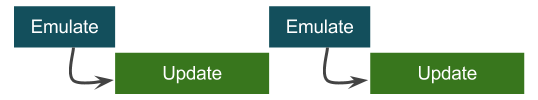
\includegraphics[width=0.4\textwidth]{img/Serial.png}}
	\caption{Sequencial Emulate and Update.}
\end{figure}
\begin{figure}[h]
	\center{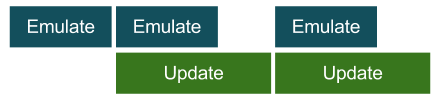
\includegraphics[width=0.4\textwidth]{img/Parallel.png}}
	\caption{Parallel Emulate and Update.}
\end{figure}

\subsubsection{Code cache}
Each time an instruction is executed the emulator is pessimistic and do all the process of decoding and executing that instruction. This includes the costly operations of reading from memory. We tried to improve this by having an instructions cache where the memory values needed to execute a given instruction where saved and then reused when the instruction was executed again. In this way we would only read from memory the needed values one time and we expected that this improves the execution of the emulator. We had some implementation issues related with the paging mechanism that does not allow us to directly associate the PC with the instruction because the original page can be switched out by another page of code. We had no time to solve this issues and so we removed the caching mechanism however we can suggest a way to turn solve this issue.\\
\indent We can solve this issue by associating the values in cache not only with the memory position but also with the number of actual the page in memory. This way we would never have to clean the cache when changing between memory pages.